\section{Main Results and Findings}\label{sec:mainResults}

\subsection{Initial Data Pre-processing}
\noindent Raw data provided was first combined into a single file and then read into a Pandas dataframe. As part of initial cleanup, 2164 duplicate rows in the dataset were identified and dropped, as shown in \autoref{fig:dropDuplicates}. 

\begin{figure}[H]
		\centering
		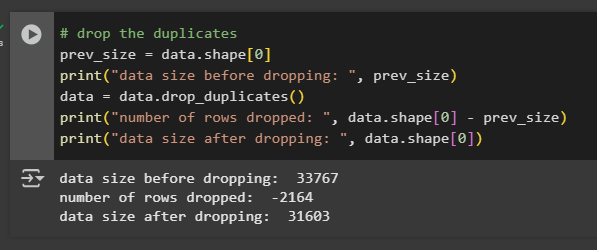
\includegraphics[scale=0.8]{figures/python_code/drop_duplicate_rows.png}
		\caption{Dropping duplicate rows}
		\label{fig:dropDuplicates}
\end{figure}

\noindent Following this, the percentage of missing values was evaluated prior to carrying out feature engineering. \autoref{fig:missingValuePercentages} displays the percentage of missing data across all raw columns:

\begin{figure}[H]
		\centering
		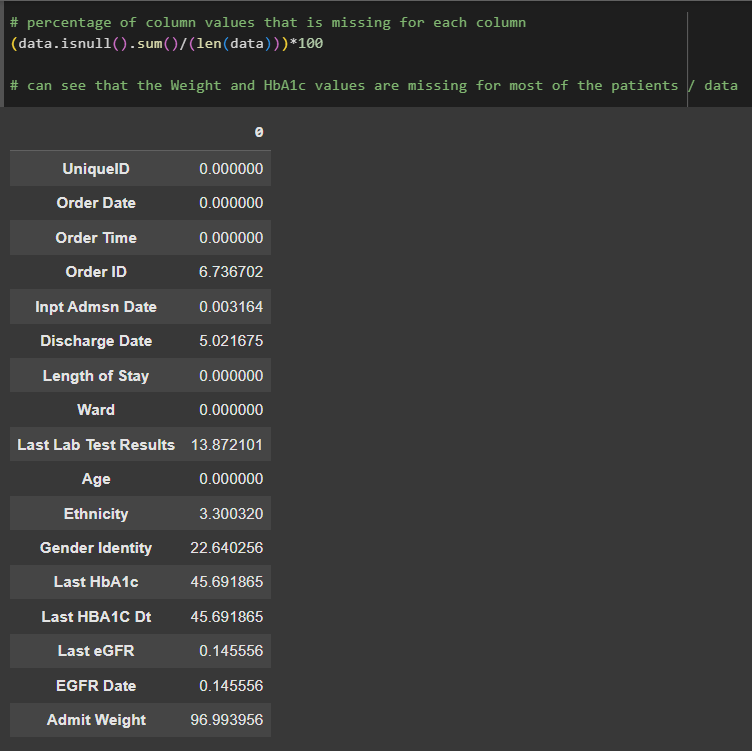
\includegraphics[scale=0.4]{figures/python_code/percent_missing_values_in_every_column.png}
		\caption{Percentage of missing values in each column}
		\label{fig:missingValuePercentages}
\end{figure}

\noindent The column Admit Weight was rendered unusable here, because it was missing 97\% of its content. Weight values cannot be calculated or imputed accurately based on the only available related features that were Age and Ethnicity, as Weight is a unique characteristic value of a patient just like Height and BMI, and to use class-based (ethnicity and age based) averages would \textbf{mislead the analysis} and produce unreliable results, so Weight is not considered in any further study hereonwards.

\subsubsection{Feature Extraction}
\noindent Next, all the columns were thoroughly examined for the exact relevant numerical values (for instance, age was given as "57kg" in the raw data as depicted in \autoref{fig:rawDataset}.) and new columns were created to store only the extracted numerical values for analysis. After this point, the usable data resembled the structure of the cleaned data as shown in \autoref{fig:cleanedDataset}.

\subsubsection{Feature Engineering}
\noindent After having acquired clear numerical values from the raw data through the newly extracted features, additional derived features were formulated based on these values. The resulting features are listed in \autoref{sec:derivedData} along with the criteria and logic used in their construction.   

\subsection{Exploratory Data Analysis}

\subsection{Interpreting model results}



% \section{Math equations}
% % \textcolor{red}{This section is for demonstration of equations, figures, tables, which is not required for the report.}
% \subsection{Maths}
% \begin{equation}\label{eq:BS}
% \frac{\D S_t}{S_t} = r \D t + \sigma \D W_t,
% \qquad S_0>0,
% \end{equation}

% The equation $\sigma = m a$ follows easily~\cite{Doe11}.


% \subsection{Glossary and acronyms}

% \newglossaryentry{Linux}
% {
%     name=latexlinux,
%     description={Is a markup language specially suited for 
% scientific documents}
% }

% \newglossaryentry{lvm}
% {
%     name=lvmformula,
%     description={A mathematical expression}
% }

% \Glspl{Linux} and other Unix operating systems are better then Windows because they support \gls{lvm} out of the box~\cite{Joh11}\insertref{A ref is missing here}. 

% \subsection{Figures}
% Here is an example~\cite{JohSil05} of how to insert a picture:

% \begin{figure}[!ht]
% \centering
% \subfigure{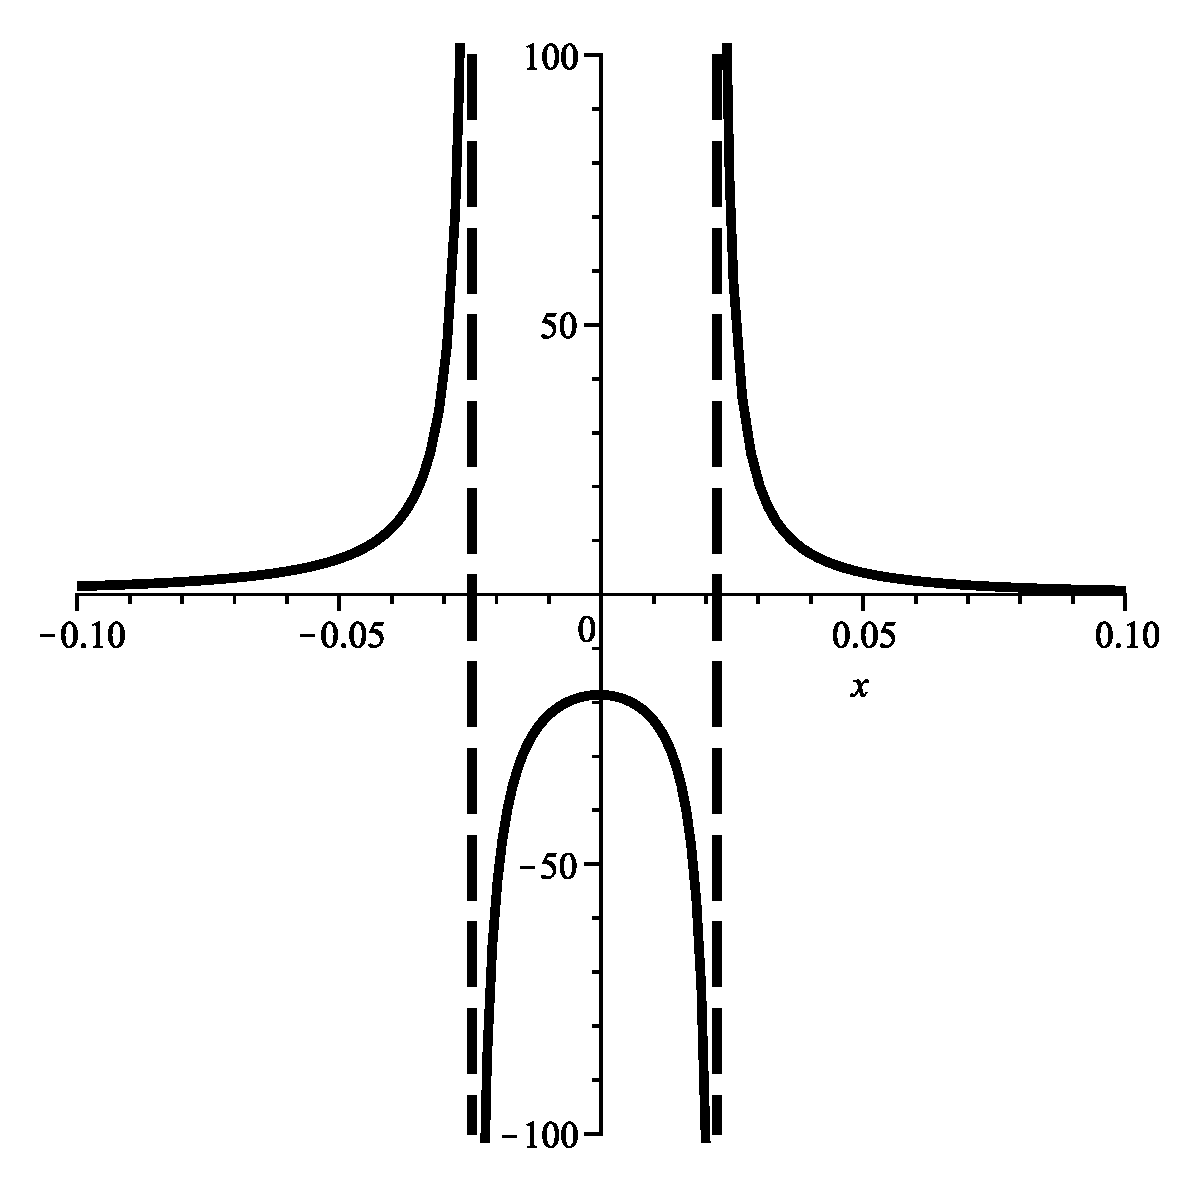
\includegraphics[scale=0.2]{figures/Picture.eps}}
% \caption{This is the caption for the figure.}
% \label{fig:Pict}
% \end{figure}


% \begin{figure}[!ht]
% \centering
% \missingfigure{If you know there will be a figure, but you still need to create it.}
% \caption{This is the caption for the figure which is not even present.}
% \label{fig:PictMis}
% \end{figure}


% Lorem ipsum dolor sit amet, consetetur sadipscing elitr, sed diam nonumy eirmod tempor invidunt ut labore et dolore magna aliquyam erat, sed diam voluptua. At vero eos et accusam et justo duo dolores et ea rebum. Stet clita kasd gubergren, no sea takimata sanctus est Lorem ipsum dolor sit amet. Lorem ipsum dolor sit amet, consetetur sadipscing elitr, sed diam nonumy eirmod tempor invidunt ut labore et dolore magna aliquyam erat, sed diam voluptua. At vero eos et accusam et justo duo dolores et ea rebum. Stet clita kasd gubergren, no sea takimata sanctus est Lorem ipsum dolor sit amet.\todo{This is a small Todo, please take care!}

% or two side-by-side pictures:

% \begin{figure}[!ht]
% \centering
% \subfigure{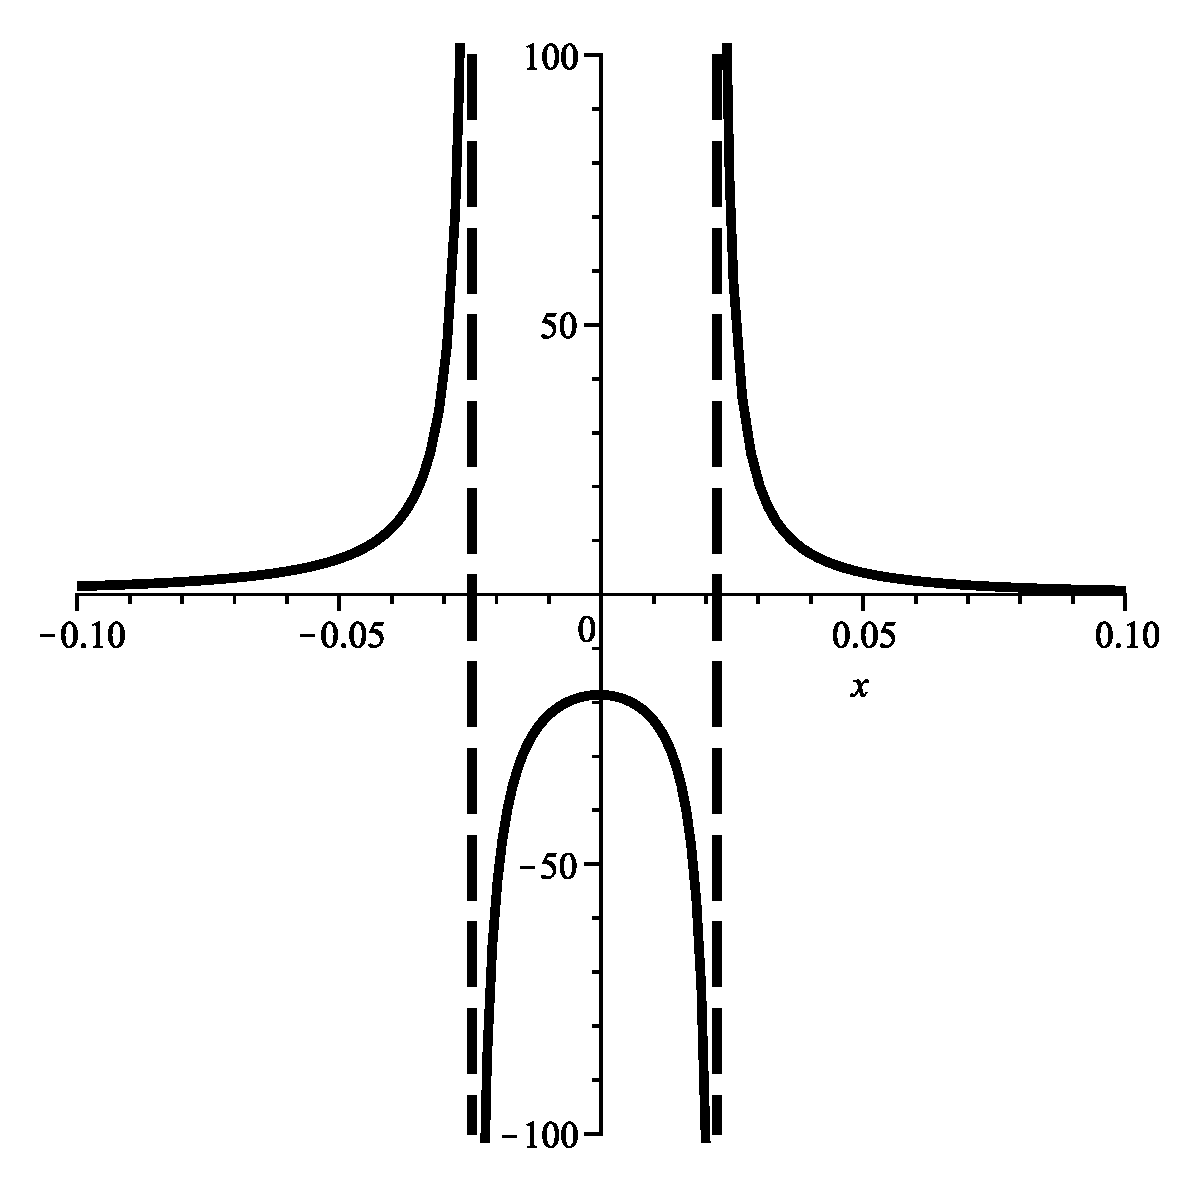
\includegraphics[scale=0.3]{figures/Picture.eps}}
% \hspace{15pt}
% \subfigure{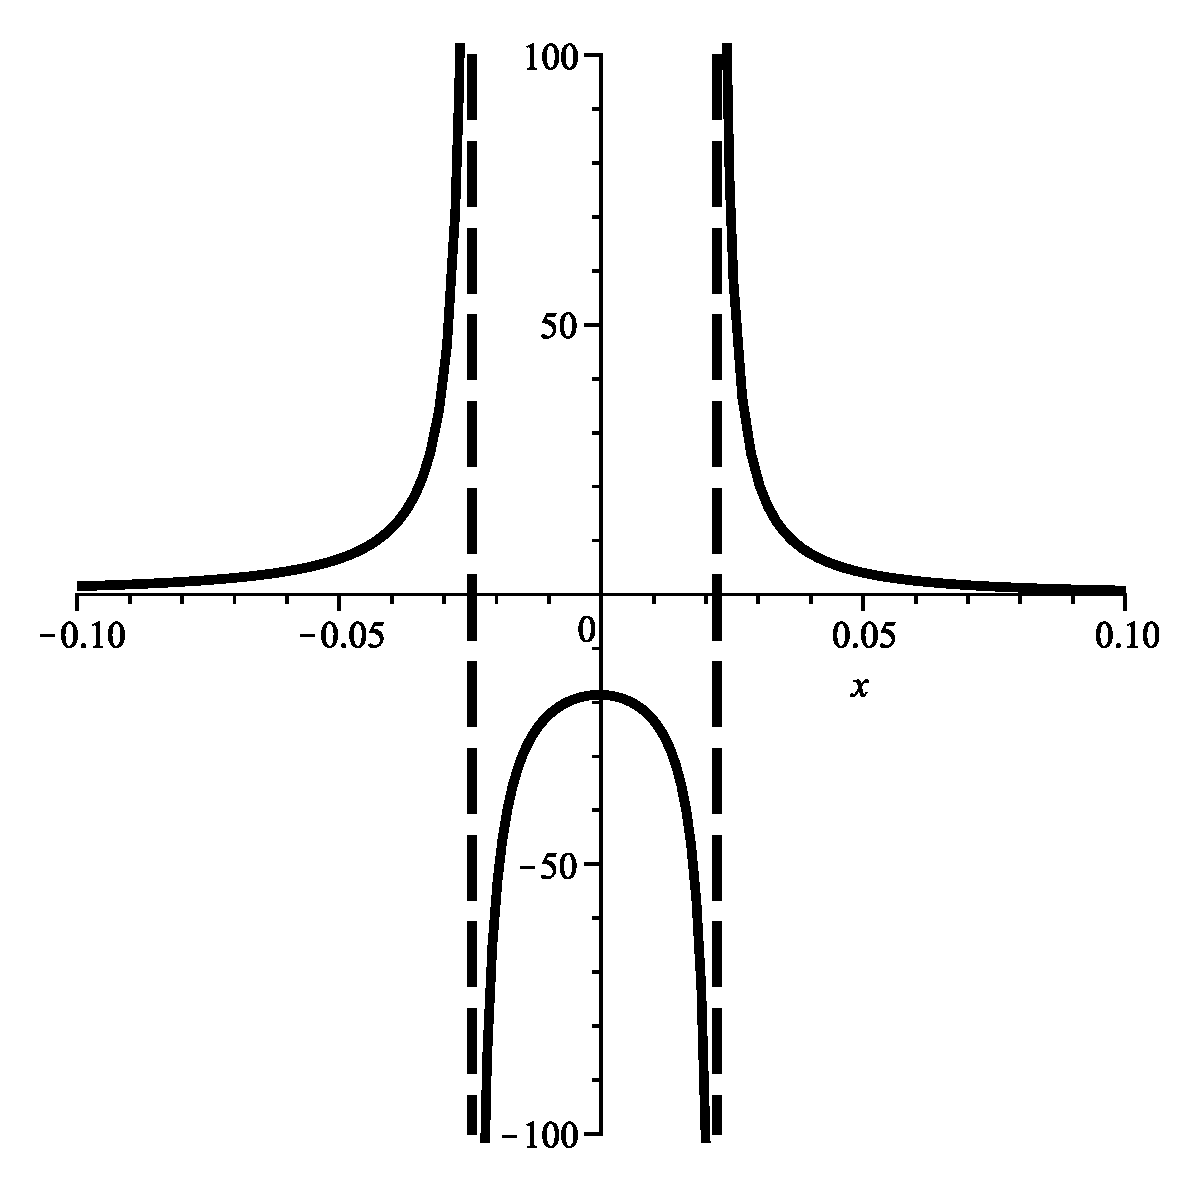
\includegraphics[scale=0.3]{figures/Picture.eps}}

% \caption{Another caption}
% \label{fig:Pict2}
% \end{figure}



% \subsection{Table}
% Lorem ipsum dolor sit amet, consetetur sadipscing elitr, sed diam nonumy eirmod tempor invidunt ut labore et dolore magna aliquyam erat, sed diam voluptua. At vero eos et accusam et justo duo dolores et ea rebum. Stet clita kasd gubergren, no sea takimata sanctus est Lorem ipsum dolor sit amet. Lorem ipsum dolor sit amet, consetetur sadipscing elitr, sed diam nonumy eirmod tempor invidunt ut labore et dolore magna aliquyam erat, sed diam voluptua. At vero eos et accusam et justo duo dolores et ea rebum. Stet clita kasd gubergren, no sea takimata sanctus est Lorem ipsum dolor sit amet\explainindetail{This needs further explanation}.
% \begin{table}[!ht]
% 	\centering
% 	\begin{tabular}{|l|rl|}
% 		\hline
% 		Something & Someother & Thing \\
%   		Seems & to be & good\\
%   		\hline
%   	\end{tabular}
%   	\caption{Random data for a table.}
% \end{table}

% Lorem ipsum dolor sit amet, consetetur sadipscing elitr, sed diam nonumy eirmod tempor invidunt ut labore et dolore magna aliquyam erat, sed diam voluptua. At vero eos et accusam et justo duo dolores et ea rebum. Stet clita kasd gubergren, no sea takimata sanctus est Lorem ipsum dolor sit amet. Lorem ipsum dolor sit amet, consetetur sadipscing elitr, sed diam nonumy eirmod tempor invidunt ut labore et dolore magna aliquyam erat, sed diam voluptua. At vero eos et accusam et justo duo dolores et ea rebum. Stet clita kasd gubergren, no sea takimata sanctus est Lorem ipsum dolor sit amet.


% \section{More Others}
% \subsection{What is calibration?}
% Here is an example of a matrix\cite{website:fermentas-lambda} in $A\in\mathcal{M}_n(\RR)$:
% $$
% A = 
% \begin{pmatrix}
% a_{11} & a_{12} & \ldots & a_{1n}\\
% a_{21} & \ddots & \ddots  & \vdots\\
% \vdots &  \ddots & \ddots  & \vdots\\
% a_{n1} &  \ldots &  \ldots & a_{1n}.
% \end{pmatrix}
% $$

% \subsection{Numerical methods for calibration}
% ...


